\documentclass[conference]{IEEEtran}
\IEEEoverridecommandlockouts
\usepackage{cite}
\usepackage{amsmath,amssymb,amsfonts}
\usepackage{algorithmic}
\usepackage{graphicx}
\usepackage{textcomp}
\usepackage{xcolor}
\usepackage{booktabs}
\usepackage{array}
\usepackage{url}
\usepackage{multirow}
\usepackage{enumitem}
\def\BibTeX{{\rm B\kern-.05em{\sc i\kern-.025em b}\kern-.08em
    T\kern-.1667em\lower.7ex\hbox{E}\kern-.125emX}}
\graphicspath{{figures/}}

\begin{document}

\title{Deep Generative Genre Remastering}

\author{\IEEEauthorblockN{Sahara Kaul}
\IEEEauthorblockA{\textit{Department of Computer Science} \\
\textit{University of Alberta}\\
Edmonton, Canada \\
sahara@ualberta.ca}
\and
\IEEEauthorblockN{Ahmed Sajid}
\IEEEauthorblockA{\textit{Department of Computer Science} \\
\textit{University of Alberta}\\
Edmonton, Canada \\
asajid2@ualberta.ca}
\and
\IEEEauthorblockN{Kelsey Pattison}
\IEEEauthorblockA{\textit{Department of Computer Science} \\
\textit{University of Alberta}\\
Edmonton, Canada \\
kpattiso@ualberta.ca}
}

\maketitle

\begin{abstract}
This report presents Deep Generative Genre Remastering (DGGR), a staged music generation system for controlled audio genre remastering. Instead of treating style transfer as direct signal repainting, the project decomposes the problem into progressively harder stages: learning a content-style representation, turning style into a controllable target space, generating accompaniment toward that target, and maintaining coherence over long-form playback. The implementation explored two reconstruction families: a codec-based latent translator using EnCodec and FiLM conditioning, and a diffusion-based mel generator using classifier-free guidance, BigVGAN-compatible mel features, and source anchoring. Long-form continuation required additional systems engineering, including overlap-prefix locking, periodic re-anchoring, stabilization blends, and a preserved-vocal hybrid production path. Quantitatively, the control stages were strong: Lab 1 reached 0.9417 style probe accuracy, 0.1083 content leakage above baseline, and 0.9299 music-gate ROC-AUC; Lab 2 reached 0.4939 silhouette, 0.8554 linear probe accuracy, and 0.8514 nearest-centroid accuracy in the 160-dimensional target space. Later stages produced locally realistic accompaniment and a usable practical workflow, but also revealed the main unresolved bottleneck: generating full, believable, stylistically distinct accompaniment over long time horizons without losing song identity or accumulating warble and drift. The project therefore succeeded most clearly as a staged control pipeline and as a practical hybrid system, while leaving long-form accompaniment generation as the primary research challenge.
\end{abstract}

\begin{IEEEkeywords}
music generation, style transfer, diffusion models, neural codecs, audio synthesis, genre remastering, long-form coherence
\end{IEEEkeywords}

\section{Introduction}
Music genre transfer looks simple when described at a distance. One begins with a source song, names a target genre, and asks a model to make the first sound like the second. The difficulty appears immediately once stronger requirements are imposed. The output should still feel like the same song. It should preserve enough structure, phrasing, and recognizable identity that the listener hears a remaster rather than a replacement. At the same time, the output should move far enough away from the source that the new genre is not merely decorative. It should sound like genuinely different accompaniment, instrumentation, or textural design rather than a thin stylistic tint laid on top of the original track.

That tension governed the entire project. If the system stays too close to the source, style transfer is weak and the result behaves like a timid filter. If the system moves too aggressively, the first thing to collapse is often the musical identity of the source. Once the output no longer feels like the same song, the system has failed the remastering objective even if the audio is superficially interesting. Much of the final system structure came from this observation: the problem was not simply to maximize stylistic distance, but to find a controllable path through a very unstable tradeoff surface.

The project therefore moved away from what we repeatedly referred to in our internal documents as a \emph{coat-of-paint} view of style transfer. In that view, a system directly distorts the source signal toward a target style and hopes that the transformed audio will preserve enough structure to remain usable. We instead treated genre remastering as a staged deconstruct-and-reconstruct problem. The project was organized around a sequence of technical questions:
\begin{enumerate}[leftmargin=1.5em]
    \item Can music be represented in a way that separates content from style strongly enough to support controlled editing?
    \item Can style be turned into a target space with usable geometry rather than a vague latent that is only measurable after the fact?
    \item Can accompaniment be regenerated toward that target using a realism-aware generator?
    \item Can those local generations survive long-form playback without seams, drift, instability accumulation, or identity collapse?
\end{enumerate}

This framing changed how failures were interpreted. In a single end-to-end system, a bad output does not reveal which part of the pipeline failed. In DGGR, each lab was designed to eliminate one ambiguity before the next stage was judged. Lab 1 removed representational ambiguity. Lab 2 removed conditioning ambiguity. Only then could later failures be attributed mainly to the generator, the sampling procedure, or the long-form continuation logic.

The final state of the project supports a stronger conclusion than a simple success-or-failure label. The project solved several foundational subproblems, established a practical production path, and narrowed the remaining work to calibration, consistency, and long-form control rather than broad uncertainty. That is the main claim of this report.

More concretely, the report makes the following contributions:
\begin{itemize}[leftmargin=1.5em]
    \item It presents a staged control pipeline for genre remastering based on disentangled representation learning, target-space construction, and conditional accompaniment generation.
    \item It shows that Labs 1 and 2 produced strong and interpretable control signals, making later generation experiments meaningfully diagnosable.
    \item It compares codec-based latent translation and diffusion-based mel generation as two different realism-control tradeoff strategies.
    \item It documents the long-form engineering layer---source anchoring, overlap prefix locking, re-anchoring, stabilization blends, and preserved-vocal mixing---that turned the strongest generator into the most usable practical workflow.
    \item It reports both metric-level and perceptual findings from the final audit, including the key lesson that stronger style movement did not always correspond to better full-song outputs.
\end{itemize}

The rest of the report follows the same logic as the project itself. We first review the work that motivated our design decisions. We then describe the DGGR pipeline and each of its labs in detail. After that we document implementation and evaluation protocol, present results by stage, and end with a discussion of why the hybrid baseline won in practice and what still remains unresolved.

\section{Related Work}
\subsection{From Superficial Style Transfer to Structured Remastering}
The most important conceptual background for DGGR is the distinction between changing the \emph{surface} of audio and changing the \emph{structure} under which a style is expressed. A recurring theme in the music style transfer literature is that many systems can produce stylistic cues without genuinely re-authoring a piece in the target style. In practical listening, that often produces outputs that resemble the source audio painted with new timbral coloration rather than rewritten arrangement or instrumentation.

Dai et al. make this ambiguity explicit in their position paper on music style transfer, arguing that the field often collapses distinct problems such as timbre transfer, performance transfer, and composition transfer into one overloaded phrase \cite{dai2018}. That framing matched our experience closely. DGGR was never just a timbre repainting system, so we needed a pipeline that could separate arrangement-level change from superficial spectral distortion.

This distinction matters more in genre remastering than in narrow timbre transfer. Genre is not only a matter of local tone color. It often involves instrumentation, groove, spectral balance, articulation, temporal density, and arrangement conventions. Earlier work on genre representation already showed that genre is a broad and unstable descriptor rather than a single acoustically grounded variable \cite{aucouturier2003}. Later deep genre-recognition systems improved classification performance substantially \cite{ghosal2018}, but those results do not by themselves imply controllable remastering. A genre-conditioned system that only perturbs the local texture of a track may achieve a classifier score without sounding like a genuine remaster. This concern motivated our emphasis on explicit control and on evaluation criteria that go beyond whether a model can make a style label more predictable.

\subsection{Disentanglement and Musical Factorization}
Disentangled representation learning provided the first major design anchor for DGGR. Hung et al. showed that timbre and composition can be separated into distinct latent variables, making it possible to manipulate one without fully rewriting the other \cite{hung2019}. Their work is directly aligned with the first-stage problem in our project: if musical content and style are not separable, then any later attempt at controlled remastering becomes ill-posed.

Yang et al. extended this line of work by explicitly separating pitch, rhythm, and chord-related content in a latent analogy framework \cite{yang2019}. That result mattered to DGGR for two reasons. First, it reinforced the idea that music is not monolithic: different musical factors must often be treated as independently controllable. Second, it suggested that representation quality should be judged not only by reconstruction but by whether downstream manipulations become interpretable.

MusicVAE further strengthened the case for structured representations by showing that hierarchical latent variables can help preserve longer-term musical organization \cite{musicvae2018}. Even though MusicVAE is primarily MIDI-oriented and therefore not a direct answer to raw audio remastering, its emphasis on long-range structure influenced our later long-form engineering decisions. The underlying message is consistent: if the representation does not respect structure, later synthesis will likely trade away global coherence for local plausibility.

\subsection{Audio Generation Backbones}
Generative models for audio have historically faced an unpleasant tradeoff between fidelity, controllability, and stability. WaveGAN demonstrated that direct adversarial waveform generation is possible, but also highlighted the difficulty of producing coherent local audio structure over time \cite{wavegan2018}. In our own project history, early raw or lightly structured generation approaches ran into exactly the kinds of problems the literature warns about: screeching, phase-related brittleness, and outputs that were technically generated but perceptually unusable.

More broadly, stable adversarial training itself required methodological fixes such as gradient-penalized Wasserstein objectives \cite{gulrajani2017}. That line of work mattered to DGGR indirectly: it clarified why adversarial waveform generation is often brittle unless the training dynamics are carefully constrained.

GANSynth addressed some of these problems by moving to spectral representations and generating magnitude plus instantaneous frequency rather than raw waveform samples \cite{gansynth2019}. This was conceptually important to DGGR because it validated the broader idea that an intermediate representation can improve generation quality. Our diffusion branch later adopted a mel-spectrogram path for similar reasons: generation becomes more stable when the model works in a representation with stronger inductive structure than raw waveform space.

At the decoding stage, BigVGAN provided a robust vocoder for translating mel representations into waveform audio across a wide range of sound types \cite{bigvgan2023}. This was valuable because it allowed the diffusion branch to focus on generating plausible mels rather than learning waveform synthesis from scratch. In parallel, EnCodec provided a different realism shortcut \cite{encodec2023}. Instead of producing an entirely new waveform representation and then decoding it, one can operate in a pretrained codec latent space and rely on the decoder as a realism prior. These two models naturally motivated our two main Lab 3 branches: codec translation and diffusion generation.

\subsection{Conditioning and Guidance}
Conditional control is central to genre remastering. The challenge is not only to generate realistic audio, but to steer that generation toward a style destination without destroying content. FiLM offered a practical way to inject target-style information into intermediate layers through feature-wise affine modulation \cite{film2018}. In DGGR, this principle was used most explicitly in the codec translator, where the generator needed to reshape a source latent trajectory under the influence of a style blueprint.

On the representation side, MERT provided a music-aware self-supervised backbone that could serve both as a style probe and as a conditioning source \cite{mert2023}. In later project iterations, MERT-based style embeddings were preferred to raw Lab 1 centroids because the latter collapsed too much in practice. This is an important example of how the project borrowed from existing models pragmatically rather than forcing every function to come from one in-house encoder.

For diffusion sampling, DDPM established the core denoising framework \cite{ddpm2020}, while classifier-free guidance gave us an explicit way to tune conditional strength without training a separate classifier \cite{cfg2021}. These tools were central in the diffusion branch because they exposed exactly the tradeoff we cared about: stronger conditioning can increase style movement, but also raises the risk of instability, over-steering, or loss of source identity.

\subsection{Editing, Anchoring, and Long-Form Coherence}
One of the clearest findings in the project is that local generation quality and full-song generation quality are different problems. This is not unique to DGGR. SDEdit formalized a useful view of guided generation: start from a meaningful input, corrupt it to a chosen noise level, and let the model reconstruct it back onto the data manifold \cite{sdedit2022}. That principle mapped neatly onto our long-form continuation problem. By periodically re-anchoring to a noised version of the source mel and forcing continuity at overlaps, we could constrain drift without completely freezing stylistic movement.

AudioLM and related large-scale generation systems demonstrate that long-range audio synthesis is possible in principle \cite{audiolm2023}, but they do not directly solve the narrow task of \emph{controlled genre remastering of an existing song}. In our setting, the model must not only produce plausible continuation, but do so while preserving a specific song's identity and moving toward a chosen target style. That combination of constraints made long-form coherence more of a systems engineering challenge than a pure generative modeling problem.

Taken together, the literature suggested a practical roadmap: separate content from style, define a structured target space, use a realism-aware generation backbone, and treat long-form continuity as its own problem. DGGR follows that roadmap closely, with the added benefit that each stage of the system was instrumented well enough that later failures could be interpreted rather than merely observed.

\section{DGGR System Overview}
\subsection{Design Principles}
Before describing the labs individually, the governing design rules should be stated explicitly:
\begin{itemize}[leftmargin=1.5em]
    \item \textbf{Control before generation.} A generator is difficult to improve if its conditioning inputs are not trustworthy.
    \item \textbf{Realism before aggressive style pressure.} Content collapse is harder to recover from than style under-shoot.
    \item \textbf{Local quality is not enough.} A convincing three-second texture does not imply a convincing full-song result.
    \item \textbf{Perceptual judgment must remain first-class.} Numeric losses and classifier outputs were useful, but they repeatedly diverged from what the audio actually sounded like.
\end{itemize}

These principles explain much of the system's later structure. They are also why the final project conclusion is more nuanced than a single ``best model'' claim.

\subsection{End-to-End Pipeline}
DGGR was implemented as a four-stage pipeline:
\begin{enumerate}[leftmargin=1.5em]
    \item \textbf{Lab 1: Deconstruction Encoder.} Learn content and style embeddings plus a music-validity gate.
    \item \textbf{Lab 2: Target Vector Space.} Build a 160-dimensional target style representation with genre centroids and measurable geometry.
    \item \textbf{Lab 3: Reconstruction.} Explore codec latent translation and diffusion-based mel generation as two different generation backbones.
    \item \textbf{Lab 4: Long-Form Coherence and Hybrid Production.} Engineer continuation stability, overlap consistency, and a preserved-vocal practical workflow.
\end{enumerate}

Conceptually, the pipeline moved from \emph{representation} to \emph{control} to \emph{generation} to \emph{survival over time}. That sequence is important. It is the main reason the project reads like a staged engineering program rather than a pile of disconnected experiments.

\begin{figure*}[t]
\centering
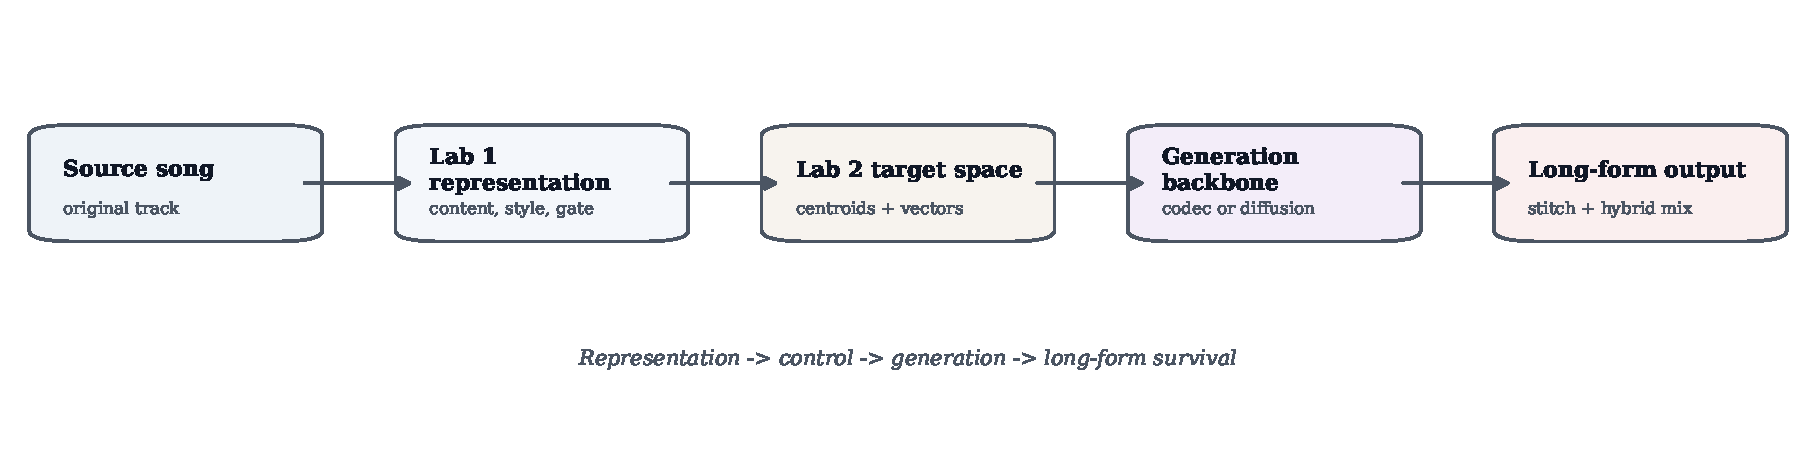
\includegraphics[width=0.96\textwidth]{dggr_pipeline_overview.pdf}
\caption{DGGR pipeline overview. The project moved from representation learning to target-space construction, then to generation, and finally to long-form stabilization and hybrid production.}
\label{fig:overview}
\end{figure*}

\section{Method}
\subsection{Lab 1: Learning a Trustworthy Musical Decomposition}
Lab 1 answered a narrow but essential question: can the system decompose music into useful internal parts? It did not aim to produce impressive audio by itself. Its value was diagnostic. When later generations sounded poor, the project needed to know whether the generator was weak or whether the representation itself had failed to learn meaningful musical structure.

The encoder operated on log-mel representations and produced three outputs:
\begin{itemize}[leftmargin=1.5em]
    \item a content code $z_{content}$ intended to preserve song identity, structure, and musically relevant continuity while suppressing style,
    \item a style code $z_{style}$ intended to retain genre-bearing and timbre-related information,
    \item a music-validity gate intended to distinguish useful musical segments from weak or non-musical supervision.
\end{itemize}

\begin{figure}[t]
\centering
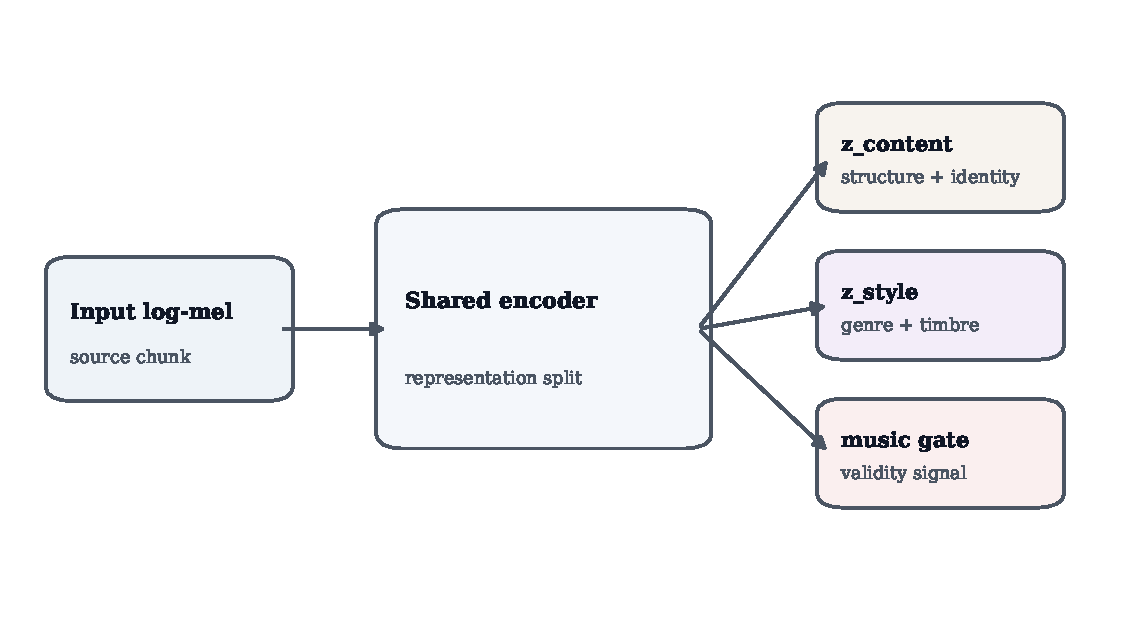
\includegraphics[width=\columnwidth]{lab1_factorization.pdf}
\caption{Lab 1 decomposition. A shared encoder produced content, style, and music-validity signals so later failures could be attributed to generation rather than representational collapse.}
\label{fig:lab1factor}
\end{figure}

The architectural idea was grounded in disentanglement. We wanted $z_{style}$ to remain explicitly style-informative while $z_{content}$ became as style-suppressed as possible. Project documentation indicates that gradient-reversal-style adversarial pressure was part of the design logic: downstream discriminators or probes should find it easy to recover style from $z_{style}$ but difficult to recover it from $z_{content}$. The music gate added a third function. Rather than treating every chunk as equally valid for downstream use, the system explicitly modeled whether the representation looked musically meaningful enough to trust.

This lab mattered for more than cleanliness of representation. It also determined how later metrics should be interpreted. If $z_{content}$ secretly carried large amounts of style information, then content preservation metrics in later labs would be misleading. If the style branch was weak, then later generation failures could still be blamed on poor control. Lab 1 therefore served as a precondition for any serious generation study.

\subsubsection{Lab 1 objective and interpretation}
The project's metric design for Lab 1 reflected those goals directly. Style probe accuracy asked whether the style branch actually retained genre signal. Content leakage above baseline asked how recoverable style still was from the content branch. Music-gate ROC-AUC asked whether the gate could rank music-like material above weaker or invalid alternatives.

The logic behind these metrics is worth stating explicitly:
\begin{itemize}[leftmargin=1.5em]
    \item High style probe accuracy does not merely mean the model learned a classifier. It means the style branch is useful as a container of style information.
    \item Low content leakage does not guarantee perfect disentanglement, but it does mean content is not simply a relabeled style embedding.
    \item High gate ROC-AUC does not solve downstream calibration automatically, but it demonstrates useful separation between musically valid and invalid segments.
\end{itemize}

By the end of Lab 1, the project's conclusion was that representation had become trustworthy enough that later failures could no longer be dismissed as total representational confusion.

\subsection{Lab 2: Turning Style Into a Target Space}
Lab 2 asked a harder question than Lab 1. It is one thing to show that style information exists somewhere in a network. It is another to turn that information into an explicit, stable, operational control target. That was the purpose of the Lab 2 target space.

The project used a 160-dimensional target vector:
\begin{equation}
\mathbf{t} = [\,\mathbf{z}_{style}; \mathbf{d}_{32}\,],
\end{equation}
where $\mathbf{z}_{style}$ is the 128-dimensional learned style representation and $\mathbf{d}_{32}$ is a 32-dimensional descriptor summarizing additional spectral characteristics used during calibration. In practice, Lab 2 harvested style vectors from many examples, filtered inliers, and estimated genre centroids. Those centroids then became concrete destinations for later generators.

This stage corrected a real failure mode. Project decision notes indicate that raw Lab 1 style centroids collapsed in practice, with high similarity between centroids limiting controllability. The move toward MERT-probe embeddings and a better separated target space therefore was not cosmetic; it was necessary to make the control signal operational.

\subsubsection{Centroids, geometry, and why they matter}
Genre centroids in DGGR were not treated as a philosophical claim that each genre has a single true point in embedding space. They were engineering anchors. The point of a centroid was to create a stable destination that could be used during conditional generation and then audited for geometry, separability, and assignment behavior.

This matters because a later generator can fail in two very different ways:
\begin{enumerate}[leftmargin=1.5em]
    \item the target space is meaningless, so the generator never had a useful destination;
    \item the target space is usable, but the generator is too conservative, too source-anchored, or too unstable to reach it.
\end{enumerate}

Lab 2 was designed to distinguish between those cases. Silhouette, linear probe accuracy, and nearest-centroid accuracy were therefore not generic machine learning scores. They were specifically chosen to tell us whether the target space had enough structure to support later conditional generation.

\subsection{Lab 3A: Codec Latent Translation}
The first serious generation branch used codec latent translation. The motivation was pragmatic. Earlier waveform-level or lightly constrained spectral generation attempts were unstable, and the project needed a path with a strong realism floor. EnCodec provided that floor. By encoding the source waveform into a pretrained latent space, editing the latents, and decoding with the pretrained decoder, the system could rely on the codec as a waveform prior.

The pipeline can be summarized as:
\begin{equation}
\begin{aligned}
\mathbf{q}_{src} &= E_{codec}(x), \\
\hat{\mathbf{q}} &= G(\mathbf{q}_{src}, z_{content}, z_{style}^{tgt}, \epsilon), \\
\hat{x} &= D_{codec}(\hat{\mathbf{q}}).
\end{aligned}
\end{equation}
Here, $\mathbf{q}_{src}$ denotes the source codec latents, $G$ is the learned translator, and $D_{codec}$ is the pretrained decoder. Conditioning included the frozen Lab 1 content representation and a target-style embedding. Noise injection was also used to encourage stochasticity and discourage trivial copying.

The translator itself used FiLM-conditioned residual blocks. In simplified form, FiLM modulation may be written as:
\begin{equation}
\mathrm{FiLM}(F \mid s)=\gamma(s)\odot F + \beta(s),
\end{equation}
where the style signal $s$ predicts channel-wise scaling and bias. In DGGR, FiLM made it possible to inject target-style information throughout the latent transformation process rather than only concatenating style at the input.

\subsubsection{Direct-output vs. residual translation}
One of the more consequential architectural choices in the codec branch was whether the translator should predict a residual correction on top of the source latents or directly output the new latent sequence. The best short-form codec run used \emph{direct-output} translation. This is a revealing detail. Residual prediction is safer because it keeps the model near the source, but it can also impose a hard ceiling on stylistic movement. Direct-output translation removed that leash. The fact that it worked best suggests that the branch needed freedom to rewrite the latent representation more aggressively, as long as content preservation was still enforced by explicit losses.

\subsubsection{Codec loss design}
The codec translator was not trained with a single objective. Project documentation describes a composite loss including:
\begin{itemize}[leftmargin=1.5em]
    \item adversarial hinge loss with a multi-scale waveform discriminator,
    \item feature matching,
    \item latent $L_1$ and latent continuity penalties,
    \item multi-resolution STFT reconstruction,
    \item content cosine preservation using $z_{content}$,
    \item style classification or probe-based style losses,
    \item push losses discouraging the source genre.
\end{itemize}

This loss stack reveals the branch's intended balance: preserve content, move style, and stay physically plausible at the waveform level. It also foreshadows a lesson that recurs later in the report: broad numeric improvement did not necessarily imply perceptual improvement. The codec branch could achieve strong style metrics while still encountering limitations in how large and convincing the remaster actually sounded.

\subsection{Lab 3B: Diffusion-Based Mel Generation}
The diffusion branch became the main realism anchor of the project. Unlike codec translation, which edits a source latent trajectory, diffusion in DGGR generated BigVGAN-compatible mel-spectrograms under content and style conditioning. The rationale was straightforward: direct generation in mel space offered a better chance of producing larger perceptual changes than a codec translator constrained by a source latent manifold.

The branch used BigVGAN-compatible 80-bin mel representations together with cached musical features such as chroma, onset envelopes, and beat-grid information. Frozen Lab 1 content and style embeddings were also provided to the model. Project documentation for the V2 diffusion model highlights several choices:
\begin{itemize}[leftmargin=1.5em]
    \item a v-prediction objective rather than simple epsilon prediction,
    \item EMA stabilization during sampling,
    \item classifier-free guidance via conditioning dropout during training and guidance during inference,
    \item separated style modulation and time/content conditioning in the network blocks.
\end{itemize}

Classifier-free guidance in simplified form may be written as:
\begin{equation}
\hat{\epsilon} = \epsilon_{uncond} + w(\epsilon_{cond} - \epsilon_{uncond}),
\end{equation}
where the guidance weight $w$ controls how strongly the target conditioning should influence the denoising trajectory. In practice, this parameter became one of the operational knobs for tuning the content-versus-style tradeoff. Higher guidance could push style harder, but also increased the risk of brittle outputs or identity loss.

\subsubsection{Why diffusion became central}
The project's final position on diffusion was not that it solved everything. It did not. Rather, diffusion became central because it established the strongest perceptual floor for accompaniment realism once wrapped in the right controls. Project notes explicitly say that later epochs often improved numeric validation loss while perceptual quality peaked earlier. That behavior is consistent with the branch's role: it was not merely an optimizer target, but a practical generation engine whose outputs had to be judged by listening.

The branch also demonstrated a key methodological lesson. A generator can be quantitatively improving while becoming perceptually smoother, thinner, or more average. This is one reason the report later devotes significant space to checkpoint selection and realism-first supervision.

\subsection{Lab 4: Long-Form Coherence and Hybrid Production}
Short-form generation was not the final problem. The hardest unresolved issue appeared when promising local outputs had to survive over time. Minutes-long generation introduced new failure modes: drift across chunk boundaries, accumulation of warble and static, weakening of song identity, and increasingly obvious mismatch between vocals and generated accompaniment.

Lab 4 addressed those problems with a combination of chunked generation and explicit continuity constraints. The core long-form approach implemented in the project combined two mechanisms:
\begin{enumerate}[leftmargin=1.5em]
    \item \textbf{SDEdit-style source anchoring.} Each chunk begins from a noised version of the source mel at timestep $t_{start}$ and is denoised toward the target condition.
    \item \textbf{Prefix-lock overlap correction.} During each DDIM step, overlap frames are overwritten using a noise-matched version of the previous chunk's tail overlap.
\end{enumerate}

This design directly reflects the project's decision record: chunked generation drifts, so the source must be reintroduced deliberately and overlap regions must be protected continuously, not just at the final waveform stitching stage.

\subsubsection{Stabilization knobs}
Even with anchoring and overlap locking, long-form stability required additional controls. The project documents the following practical knobs:
\begin{itemize}[leftmargin=1.5em]
    \item periodic re-anchoring,
    \item time/frequency mel smoothing,
    \item global source-mel blending,
    \item extra high-frequency source blending,
    \item style-strength mixing between source and target style embeddings.
\end{itemize}

These controls make the branch look less like a pure model and more like a system. That is the correct interpretation. By this stage the remaining problem was not only what the generator could do locally, but how to constrain it over time without freezing it into a near-identity copy.

\subsubsection{Why the hybrid workflow won}
The most practical system in the project preserved vocals and concentrated generative freedom on the accompaniment. This decision deserves explicit defense because it can be misread as a shortcut. It was, instead, a principled response to observed model weakness. Vocals were among the most fragile components under aggressive generation, while accompaniment carried more of the genre-shift burden and tolerated larger edits. Preserving vocals therefore improved intelligibility, sync, and practical listenability while still allowing the system to explore new accompaniment textures.

This is one of the clearest systems-engineering outcomes of the project. The best practical path was not ``one magical end-to-end model.'' It was a layered solution that protected the most fragile component and concentrated model freedom where style movement mattered most.

\begin{figure}[t]
\centering
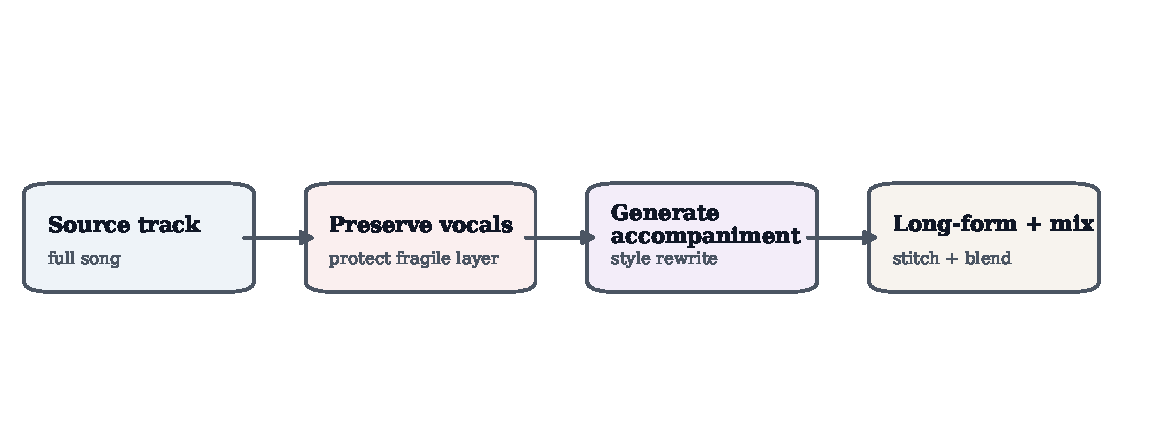
\includegraphics[width=\columnwidth]{hybrid_workflow.pdf}
\caption{Hybrid production workflow used in the final practical path. Vocals were preserved while generative freedom was concentrated on accompaniment and long-form support.}
\label{fig:hybridflow}
\end{figure}

\section{Implementation Overview and Experimental Protocol}
\subsection{Implementation Structure and Artifacts}
DGGR was implemented as an experiment-driven system rather than a single training script. This had important consequences for reproducibility and evaluation. The project separates explanation documents, reference material, decision records, and lab-specific implementations. Large datasets are intentionally not committed, but data schemas, caches, manifests, and run folders are documented clearly enough to reconstruct the pipeline on a local machine.

Manifest CSVs store audio paths, dataset-source identifiers, and genre-bucket labels. Later labs consume cached derivatives rather than raw audio directly. Lab 2 writes harvested embeddings, centroid files, validation summaries, and vector indices. The codec branch stores EnCodec latents, frozen Lab 1 embeddings, and optional MERT features. The diffusion branch stores mel arrays, conditioning features, genre indices, and metadata. Long-form outputs include rendered full-song waveforms, chunk-level exports, and coherence diagnostics.

This artifact-oriented structure matters because the project's evaluation increasingly depended on being able to compare runs after training, not just during training. Much of the final project insight came from audits, sweep outputs, and historical run comparisons rather than from one end-to-end training log.

\subsection{Genre Buckets and Data Assumptions}
The project uses broad genre buckets rather than a claim of definitive music ontology. This is a pragmatic choice. The goal was to define categories broad enough to learn, distinct enough to benchmark, and noisy enough to expose failure modes. Examples such as \texttt{hiphop\_xtc} and \texttt{baroque\_classical} show that some categories were intentionally merged into practical engineering buckets rather than treated as pure taxonomic labels.

This matters when interpreting style separation. If two target genres remain too similar in output space, that does not automatically imply the target-space concept failed. It may instead mean the generator was over-anchored, too conservative, or too weakly incentivized to move.

\subsection{Evaluation Philosophy}
The project used different evidence at different stages. Early labs were primarily metric-driven because they were designed to establish internal structure and control. Later generation labs relied more heavily on perceptual judgment, targeted audits, and qualitative comparisons because the system repeatedly encountered disagreement between optimization metrics and listening quality.

This led to a practical evaluation philosophy:
\begin{itemize}[leftmargin=1.5em]
    \item \textbf{Lab 1 and Lab 2:} metrics are central because they answer structural questions.
    \item \textbf{Codec and diffusion short-form generation:} metrics are useful, but only if interpreted alongside audio.
    \item \textbf{Long-form generation and late model families:} perceptual audits are indispensable, because structure, fullness, vocal fit, and long-range realism are only partially captured by scalar metrics.
\end{itemize}

\subsection{Metric Definitions}
The project includes a dedicated metrics reference, which makes it possible to report metric values without stripping them of meaning. The key metrics used in this report are summarized in Table~\ref{tab:metricdefs}.

\begin{table}[t]
\caption{Core metrics and their intended interpretation.}
\label{tab:metricdefs}
\centering
\small
\begin{tabular}{@{}p{1.8cm}p{2.0cm}p{2.6cm}@{}}
\toprule
\textbf{Stage} & \textbf{Metric} & \textbf{Purpose} \\
\midrule
Lab 1 & Style probe accuracy & Tests whether $z_{style}$ retains genre signal \\
Lab 1 & Content leakage & Tests whether style remains recoverable from $z_{content}$ \\
Lab 1 & Gate ROC-AUC & Tests music-vs-nonmusic separation \\
Lab 2 & Silhouette & Measures target-space cluster geometry \\
Lab 2 & Linear probe accuracy & Measures linear genre separability \\
Lab 2 & Nearest-centroid accuracy & Tests whether centroids behave as class anchors \\
Codec & MPS & Content preservation proxy via content-code cosine \\
Codec & Style confidence / accuracy & Target-style movement and classification correctness \\
Long-form & Boundary mel MSE / dB proxy & Seam diagnostics across chunk boundaries \\
Audit & Fullness, structure, warble, confidence & Perceptual proxy family for final model comparison \\
\bottomrule
\end{tabular}
\end{table}

The existence of these metrics does not mean the project reduced listening quality to a dashboard. In fact the opposite happened. The metrics were helpful precisely because they made it easier to see when a branch was winning numerically while sounding worse perceptually.

\subsection{Checkpoint Selection and Realism Supervision}
One of the project's more mature engineering ideas was the realism supervisor. The project recognized that main training metrics often revealed whether content survived and whether style moved at all, but they did \emph{not} reliably reveal whether the audio sounded natural. As a result, checkpoint ranking later incorporated realism-oriented quantities such as Fr\'echet distance over MERT embeddings and target-reference spectral alignment measures. This did not eliminate listening, but it reduced the number of checkpoints that required human inspection.

This practical detail shows how the evaluation protocol evolved. The project did not merely train models and pick the numerically best one. It built a multi-stage filtering process: first eliminate obviously bad checkpoints, then apply realism gates, and finally listen to a smaller candidate set.

\subsection{Practical Training Workflow}
The sample paper we used as a structural reference spends significant space explaining how experiments were actually run, not only what the final numbers were. That level of implementation detail matters here as well because DGGR was not a one-pass training pipeline. Every major stage relied on a practical workflow designed around expensive generation and expensive listening.

The project converged on the following practical workflow:
\begin{enumerate}[leftmargin=1.5em]
    \item build or refresh the relevant cache for the current lab,
    \item train a short probe run to reject obviously weak ideas,
    \item evaluate checkpoints on a fixed transfer plan so that comparisons are fair,
    \item rank checkpoints using realism and movement criteria,
    \item listen only to a smaller candidate set,
    \item launch the longer run only after the previous stages indicate the branch is worth further investment.
\end{enumerate}

This workflow may sound mundane, but it is one of the reasons the project remained interpretable. Without fixed transfer plans, later checkpoints become hard to compare because they may be evaluated on different source-target pairs. Without realism-first gating, the listening workload becomes too large and too noisy. Without short probe runs, the project would have spent too much time fully training branches that were already weak after only a limited number of epochs. The central engineering lesson is simple: a generative-audio experiment pipeline needs a search strategy, not only a model definition.

\subsection{Implementation Details and Practical Constraints}
The sample paper also contains a dedicated implementation-details subsection, and DGGR benefits from the same treatment. The project was built under realistic time and compute constraints. That influenced several major decisions.

First, the project leaned heavily on caching. Lab 2 harvested embeddings and wrote validation summaries rather than re-computing feature geometry from scratch on every run. The codec and diffusion branches both cached their conditioning features, allowing model iteration without repeating expensive preprocessing. This is not just a convenience detail. Caching made it feasible to treat Labs 1 and 2 as reusable infrastructure instead of retraining or re-harvesting everything whenever a generation branch changed.

Second, the project made deliberate use of pretrained models where it was rational to do so. EnCodec was adopted as a decoder guardrail because earlier raw waveform and spectrogram GAN approaches were brittle. MERT was adopted as a style backbone because raw Lab 1 centroids collapsed too much in practice. BigVGAN compatibility shaped the diffusion branch because it provided a reliable waveform reconstruction target. These decisions reduced the amount of instability the project had to solve from scratch and allowed effort to be spent on the actual remastering problem.

Third, the project increasingly separated \emph{training metrics} from \emph{selection metrics}. This is an underappreciated implementation choice. A model can be trained on one objective and selected with another. In DGGR, main training losses determined whether a branch was learning anything useful at all, while realism supervisors, audit scripts, and listening panels decided which checkpoints were worth keeping. The project's late maturity came largely from accepting that those two layers should not be collapsed into one number.

Finally, the project had to work within the practical limitation that the most expensive part of the system was not always training. Long-form generation, checkpoint sweeps, and perceptual review were themselves costly. That is one reason later audit documents repeatedly mention overnight sweeps, short rejection probes, and careful promotion criteria for new branches. In this sense the project became not only a collection of models but an operating procedure for making controlled decisions under limited time.

\section{Experiments and Results}
\subsection{Lab 1: Representation Learning Results}
Lab 1 produced some of the cleanest successes in the entire project. The core results are shown in Table~\ref{tab:foundation}.

\begin{table}[t]
\caption{Foundation results from Labs 1 and 2.}
\label{tab:foundation}
\centering
\small
\begin{tabular}{@{}p{1.6cm}p{2.4cm}p{1.1cm}@{}}
\toprule
\textbf{Stage} & \textbf{Metric} & \textbf{Value} \\
\midrule
Lab 1 & Style probe accuracy & 0.9417 \\
Lab 1 & Content leakage above baseline & 0.1083 \\
Lab 1 & Music gate ROC-AUC & 0.9299 \\
Lab 2 & Silhouette (cosine) & 0.4939 \\
Lab 2 & Linear probe accuracy & 0.8554 \\
Lab 2 & Nearest-centroid accuracy & 0.8514 \\
\bottomrule
\end{tabular}
\end{table}

These values are meaningful because they match the lab's original design goals. A 0.9417 style probe accuracy indicates that the style branch was strongly informative. A content leakage value of 0.1083, while not zero, is comfortably below the project's own warning threshold and suggests that $z_{content}$ was substantially style-suppressed. A gate ROC-AUC of 0.9299 indicates that the music-validity head was doing real ranking work and was not merely a noisy add-on.

The practical implication is that Lab 1 stopped representation from being the default excuse for failure. Once this stage passed, later generation problems had to be treated as failures of control, generation, or long-form engineering rather than total latent collapse.

\subsection{Lab 2: Target-Space Calibration Results}
Lab 2 was the other clear structural win. The target space reached 0.4939 silhouette, 0.8554 linear probe accuracy, and 0.8514 nearest-centroid accuracy. These are not just respectable classification numbers; they imply that the 160-dimensional style-target space had usable geometry.

\begin{figure}[t]
\centering

\includegraphics[width=\columnwidth]{lab2_tsne.png}
\caption{Lab 2 target-space visualization. The learned target vectors form meaningful cluster structure, supporting the use of centroid-style conditioning.}
\label{fig:tsne}
\end{figure}

Fig.~\ref{fig:tsne} supports that same conclusion visually. The target vectors are not a single tangled cloud. They exhibit interpretable cluster structure, which is exactly what later conditioning required. This is why the final project summary repeatedly emphasizes that Labs 1 and 2 \emph{worked}. They are not where the system's later perceptual failures originate.

\subsection{Codec Branch: Short-Form Translation Results}
The codec branch produced the earliest convincing evidence that controlled reconstruction was possible. The best run, \texttt{run1055}, reached:
\begin{itemize}[leftmargin=1.5em]
    \item MPS = 0.9565,
    \item style confidence = 0.8940,
    \item style accuracy = 0.9492.
\end{itemize}

Within the lab's own framing, these are strong results. They indicate that the branch was able to push target-style evidence while preserving content well enough to exceed the project thresholds. The use of MERT-probe embeddings and direct-output translation was especially important. Project decision notes indicate that this combination improved style separability in conditioning space and removed an architectural cap on edit magnitude.

At the same time, the codec branch did not become the final production backbone. The reason was not that the branch failed completely. Rather, it revealed a ceiling: the EnCodec latent manifold protected realism, but it also limited how far the accompaniment could be perceptually rewritten. This is why codec remained important in the story as a proof-of-possibility branch, but diffusion became the stronger realism anchor for later work.

\begin{figure}[t]
\centering
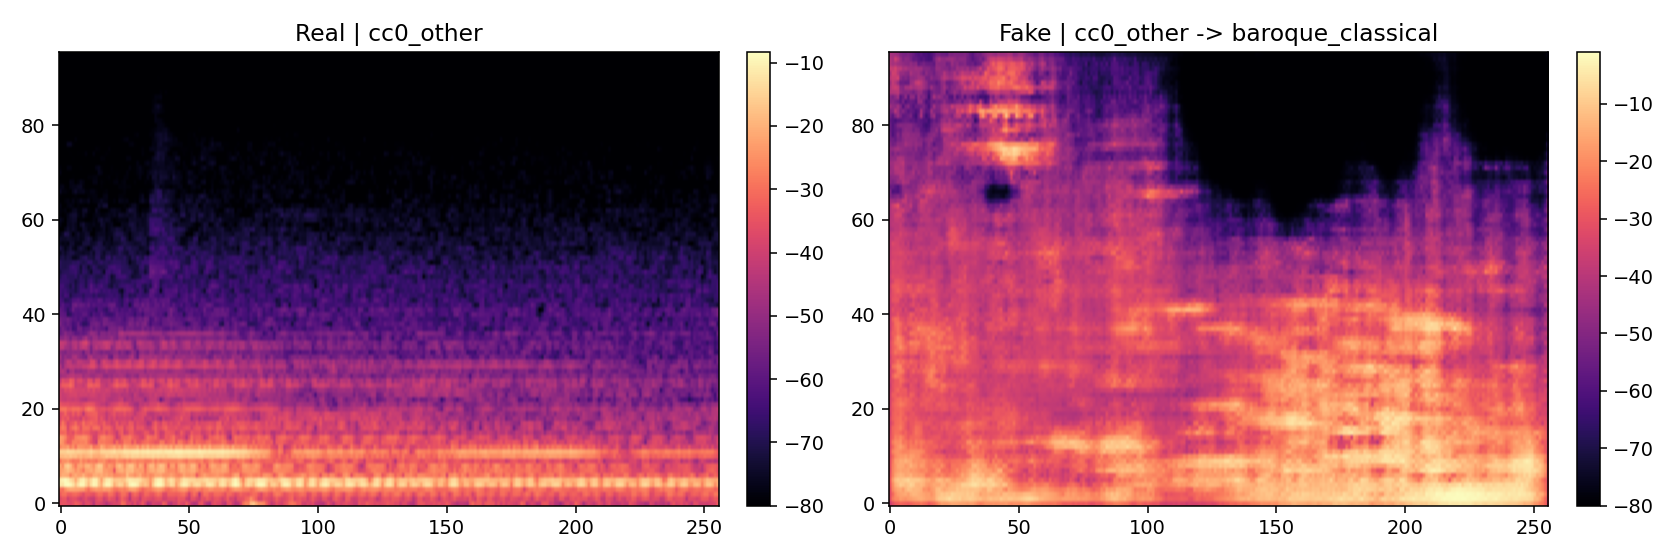
\includegraphics[width=\columnwidth]{codec_spectrogram_example.png}
\caption{Representative codec-branch spectrogram comparison from the project. The branch could preserve structure while producing a visibly different target-conditioned accompaniment, but perceptual rewrite strength still had a ceiling.}
\label{fig:codecexample}
\end{figure}

\subsection{Diffusion Branch: Checkpoints, Realism, and the Central Tradeoff}
The diffusion branch produced one of the report's most instructive results: the best numerical checkpoint was not the best listening checkpoint. In the V2 run, epoch 18 achieved the best validation loss of 0.0386, while epoch 6---with validation loss 0.0442---was selected as the best subjective checkpoint for generation.

\begin{figure}[t]
\centering

\includegraphics[width=\columnwidth]{diffusion_v2_curve.png}
\caption{Diffusion V2 validation curve. Later training reduced the scalar loss, but earlier checkpoints produced better perceived audio quality.}
\label{fig:diffcurve}
\end{figure}

This is not a minor detail. It shows why later stages of the project stopped treating scalar optimization as the whole story. The diffusion branch could continue improving by loss while becoming smoother, thinner, or less musically satisfying. This gap between optimization and listening is one of the main reasons the project later introduced realism supervision and stronger human auditing.

The diffusion branch also made the project's central tradeoff more obvious. Short local generations could sound realistic and genre-aware, but stronger style pressure increased the risk of identity collapse. Weak style pressure preserved the song but made target genres sound too similar. This tension appears throughout the final project state and is one of the clearest project-level conclusions.

\subsection{Long-Form Coherence Results}
Lab 4 provided the point at which the project's remaining bottleneck became precise. Long-form generation was evaluated with seam diagnostics such as mean boundary mel MSE and a dB-scale boundary discontinuity proxy. For the main full-song test, the project reports:
\begin{itemize}[leftmargin=1.5em]
    \item boundary mel MSE mean = 0.0018347,
    \item boundary discontinuity mean = 2.8691 dB,
    \item 64 chunks over a 160-second test.
\end{itemize}

These values are informative because they show that hard seam breaks were not the only problem. In fact, the project's own interpretation was that the main remaining issues were perceptual accumulation effects: warble, static, thinning of accompaniment body, and gradual identity drift. In other words, the system learned how to avoid catastrophic stitching failures more quickly than it learned how to sustain believable accompaniment over time.

\begin{figure*}[t]
\centering

\includegraphics[width=0.94\textwidth]{longform_comparison.png}
\caption{Long-form comparison figure from the project materials. The key lesson is that local quality did not automatically survive full-song continuation.}
\label{fig:longform}
\end{figure*}

Fig.~\ref{fig:longform} captures the practical version of this lesson. A model can generate promising local texture and still fail as a song-level system. That redefined the project's center of gravity. The difficult problem was no longer ``make the generator sound better locally.'' It became ``make the generator survive time.''

\subsection{Hybrid Production Results}
The strongest practical outputs in the project came from the late hybrid/source-conditioned family with vocal preservation and sync-safe backing generation. Project notes summarize its strengths clearly:
\begin{itemize}[leftmargin=1.5em]
    \item preserved content well,
    \item kept vocals clear enough to be practically usable,
    \item established the best vocal/accompaniment fit,
    \item provided the strongest overall listenability floor.
\end{itemize}

Its weaknesses were equally clear:
\begin{itemize}[leftmargin=1.5em]
    \item target styles remained too similar,
    \item accompaniment often sounded filtered rather than newly authored,
    \item genre movement was present but weaker than desired.
\end{itemize}

This duality explains why the hybrid system deserves careful reporting. It was the best practical path, but not the final research victory. It won because it was usable and believable, not because it maximized genre separation.

\subsection{Later Model Families and Final Audit}
After establishing the hybrid baseline, the project explored several later model families intended to break the source-conditioned ceiling. These included:
\begin{itemize}[leftmargin=1.5em]
    \item scratch retrieval-conditioned accompaniment models,
    \item sourcehint retrieval,
    \item aggressive pretrained EnCodec variants,
    \item retrieval + pretrained blends,
    \item scratch structure diffusion,
    \item later body-style retrieval variants.
\end{itemize}

The final audit did not present these as an experiment graveyard. Instead, it treated them as controlled attempts to turn different knobs: push style harder, weaken source anchoring, add retrieval, or retrain for fuller accompaniment.

Table~\ref{tab:audit} summarizes the main quantitative comparison reported in the perceptual audit.

\begin{table}[t]
\caption{Later branch comparison from the final perceptual audit. Higher confidence/fullness/structure are better; lower warble is better.}
\label{tab:audit}
\centering
\small
\begin{tabular}{@{}p{2.0cm}cccc@{}}
\toprule
\textbf{Branch} & \textbf{Conf.} & \textbf{Full.} & \textbf{Struct.} & \textbf{Warble} \\
\midrule
Scratch retrieval & 0.4410 & 0.5872 & 0.0754 & 0.0090 \\
Sourcehint retrieval & 0.3333 & 0.6296 & 0.0997 & 0.0113 \\
Pretrained EnCodec & 0.3866 & 0.6250 & 0.0473 & 0.0246 \\
Retrieval + pretrained & 0.4509 & 0.5909 & 0.0697 & 0.0095 \\
Scratch structure diff. & 0.9943 & 0.7949 & 0.0505 & 0.0271 \\
\bottomrule
\end{tabular}
\end{table}

These numbers are revealing precisely because they do \emph{not} settle the matter automatically. The scratch retrieval family was the strongest of the genuinely new model families. It improved style movement more honestly than the hybrid baseline and attacked source timbre leakage directly. Yet the audit still concluded that its accompaniment was not full or believable enough to replace the hybrid path. The retrieval + pretrained blend looked slightly stronger on the judge, but listening suggested thinner instrumentation, worse song fit, and poorer vocal/accompaniment cohesion. The scratch structure diffusion family nearly saturated target confidence, but the project explicitly labeled that result a metric illusion because the branch did not deliver trustworthy arrangement quality.

\begin{figure}[t]
\centering

\includegraphics[width=\columnwidth]{metrics_dashboard.png}
\caption{Dashboard-style summary of late-branch evaluation. The recurring pattern was that stronger apparent style movement did not automatically yield better practical outputs.}
\label{fig:dashboard}
\end{figure}

This outcome matters because the project did not merely identify failed models. It established \emph{why} they failed and which metrics were misaligned with perceptual quality.

\subsection{What the Results Collectively Show}
Taken together, the experiments support the following conclusions:
\begin{enumerate}[leftmargin=1.5em]
    \item Labs 1 and 2 succeeded in building a trustworthy control foundation.
    \item The codec branch proved that controlled latent reconstruction was possible and could preserve content strongly.
    \item The diffusion branch became the strongest realism anchor, even though it required careful checkpoint selection and long-form support.
    \item Hybrid vocal preservation was not a hack in the negative sense; it was the most effective systems response to the actual failure modes of the generators.
    \item The main unresolved problem is not whether the system can ever sound realistic locally. It is whether it can generate full, believable, stylistically distinct accompaniment over long time horizons while preserving song identity.
\end{enumerate}

\subsection{What Each Late Family Improved and What It Broke}
One of the most useful ways to summarize the second half of the project is not by naming runs, but by asking what each family changed in the tradeoff. Table~\ref{tab:familytradeoffs} compresses that logic.

\begin{table*}[t]
\caption{Late-family tradeoffs distilled from the final project analysis and perceptual audit documents.}
\label{tab:familytradeoffs}
\centering
\small
\begin{tabular}{@{}p{3.2cm}p{5.5cm}p{6.0cm}@{}}
\toprule
\textbf{Family} & \textbf{What improved} & \textbf{What broke or remained weak} \\
\midrule
Late hybrid/source-conditioned baseline & Best overall listenability, strongest vocal clarity and sync, strongest song fit, strongest practical production floor & Target styles remained too similar, accompaniment often sounded edited rather than newly authored, style movement under-shot the desired target \\
\addlinespace
Scratch retrieval family & More honest genre movement, better attack on source timbre leakage, strongest of the genuinely new branches & Arrangements still felt thin, accompaniment body remained weak, did not beat the hybrid baseline on overall musical satisfaction \\
\addlinespace
Sourcehint retrieval family & Middle-ground branch with decent song fit and somewhat improved texture variety & Target separation stayed weak, not strong enough to justify as the lead system, still lacked convincing accompaniment authorship \\
\addlinespace
Aggressive pretrained EnCodec family & Some target-style confidence improvement, useful stress test of stronger editing pressure & Warble was worse, structure weakened, some target genres degraded badly, especially in more delicate styles such as baroque/classical and lo-fi \\
\addlinespace
Retrieval + pretrained blend & Slight numerical gains on some judge outputs, more explicit style movement than the safer baseline & Regressed perceptually: thinner instrumentation, worse song fit, worse vocal/accompaniment cohesion, stronger movement without convincing musical body \\
\addlinespace
Scratch structure diffusion family & Extremely high target-confidence scores, strong headline numbers on paper & Almost certainly over-rewarded by the judge, weak structure retention, poor evidence of believable arrangement, high confidence did not correspond to trustworthy listening quality \\
\bottomrule
\end{tabular}
\end{table*}

This table is central to understanding the project honestly. The later families were not random failures; each one exposed a different knob in the system. The scratch retrieval family showed that style movement could be pushed more honestly than in the old baseline. The aggressive pretrained family showed that simply editing harder was not enough if structure and warble deteriorated. The retrieval-plus-pretrained blend showed that judge improvements are not the same thing as musical improvement. The scratch structure family showed that saturated confidence can be almost meaningless if the arrangement no longer sounds trustworthy.

Framed this way, the project's trajectory becomes much clearer. The project did not merely discover that ``later models failed.'' It discovered that the remaining challenge is not just moving farther in style space. It is doing so while maintaining enough fullness, arrangement plausibility, and song fit that the result still reads as a remaster of the same musical object.

\begin{figure}[t]
\centering
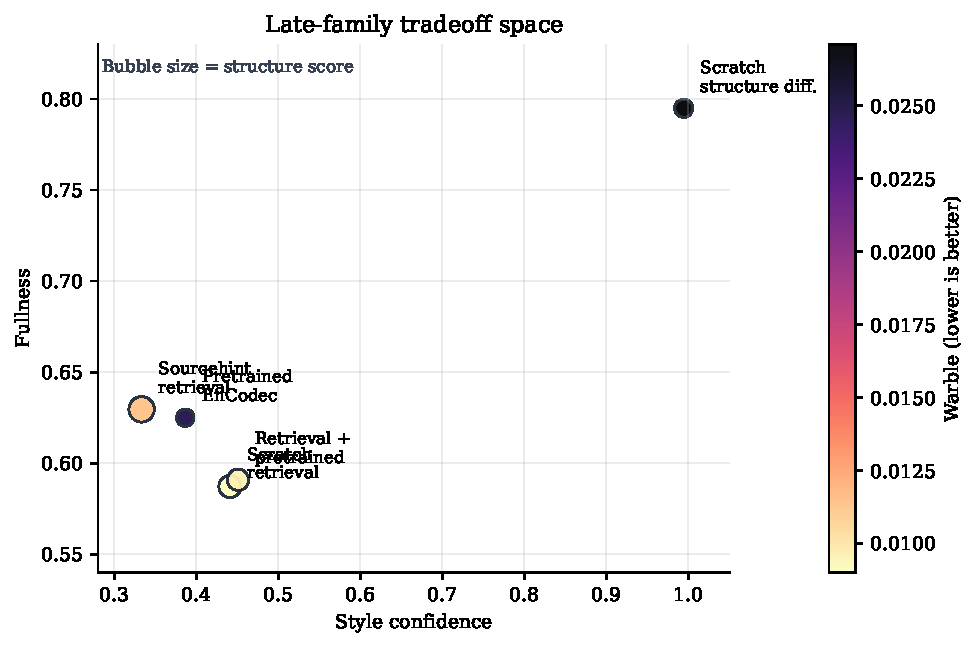
\includegraphics[width=\columnwidth]{late_family_tradeoff_scatter.pdf}
\caption{Late-family tradeoff plot derived from the final perceptual audit. Confidence, fullness, structure, and warble did not improve together, which is why no single scalar metric could summarize the later branches correctly.}
\label{fig:latefamilyscatter}
\end{figure}

\subsection{Failure Modes Observed Repeatedly in Listening}
The audit documents repeatedly converge on a small set of perceptual failure modes. These are worth naming explicitly because they organize the second half of the project more cleanly than many of the run names do.

\textbf{Style under-shoot.} The safest branches preserved the song well but left target genres too similar. This is the failure mode of the strongest practical baseline.

\textbf{Identity collapse.} Some aggressive branches created more stylistic movement, but the output stopped feeling like the same song. The result could be interesting audio without being successful remastering.

\textbf{Thin or hollow accompaniment.} Several new-model families improved movement without generating accompaniment that felt full, grounded, or richly instrumented. This is one of the strongest reasons the hybrid baseline remained ahead.

\textbf{Vocal/accompaniment mismatch.} Even when accompaniment movement improved, the blend with vocals often deteriorated. In practice, this made the output less convincing than a more conservative branch with better alignment.

\textbf{Metric illusion.} Some families achieved impressive target-confidence numbers that did not survive perceptual scrutiny. This is one of the most important warnings for future work: a style judge can be directionally useful while still being profoundly incomplete.

These recurring failures are exactly why the report should emphasize engineering process and bottleneck localization rather than treating the remaining work as vague polishing. The project ended with a specific diagnosis and a more mature control framework.

\section{Discussion}
\subsection{Why the Hybrid Baseline Won}
The late hybrid/source-conditioned path won because it optimized the right objective for the stage the project had reached. By the time the system converged on that path, it had already learned that raw style movement was not the same thing as usable remastering. The hybrid system preserved the song well, kept vocals synchronized and intelligible, and produced accompaniment that was believable enough to support presentation and demonstration. It did not push style as hard as later retrieval-heavy branches, but it consistently avoided the worst perceptual regressions that those branches introduced.

The engineering lesson is straightforward: an explicit hybrid step does not make a system less legitimate. It makes the system more practical when different parts of the signal fail in different ways.

\subsection{Practical Ranking of Branch Families}
One place where the project became unusually clear by the end was the ranking of branch families by practical usefulness. The audit documents do not merely list runs; they identify which branches are worth using, which are worth researching further, and which should be considered misleading or rejected. That ranking is summarized in Table~\ref{tab:ranking}.

\begin{table}[t]
\caption{Final branch ranking by practical usefulness, based on the project's end-state audit.}
\label{tab:ranking}
\centering
\small
\begin{tabular}{@{}p{1.0cm}p{5.4cm}@{}}
\toprule
\textbf{Tier} & \textbf{Branch family} \\
\midrule
1 & Late hybrid/source-conditioned path with vocal preservation and sync-safe accompaniment \\
1 & Offline-optimized best checkpoint family used as a strong non-hybrid practical reference \\
2 & Scratch retrieval family and later body-style retrieval variant as the best current research branches \\
2 & Aggressive pretrained EnCodec family as a useful but weaker exploratory branch \\
3 & Retrieval + pretrained blend production \\
3 & Scratch structure diffusion family \\
3 & Broad late fine-tune families that improved loss but damaged perceptual quality \\
\bottomrule
\end{tabular}
\end{table}

This ranking captures the project's central engineering judgment. The hybrid family wins in practice. Retrieval remains the most promising new-model direction. Several branches looked strong on narrow metrics but should not be promoted without stronger perceptual evidence. Preserving this hierarchy matters because otherwise the project can read like an undifferentiated pile of experiments rather than a system that learned how to reject bad directions.

\subsection{Lab-by-Lab Lessons}
Another way to summarize the project clearly is to state what each lab solved and what bottleneck it exposed next.

\textbf{Lab 1} solved ambiguity about whether the system had learned meaningful musical structure at all. Once its metrics were strong, representational collapse stopped being the default explanation for every later failure.

\textbf{Lab 2} solved ambiguity about whether the target condition was meaningful. Once the target vectors and centroids had usable geometry, later style underperformance could no longer be blamed entirely on the target space.

\textbf{Lab 3 codec} proved that controlled reconstruction was possible in a realism-protected latent space. It also revealed that a realism guardrail can become a style-magnitude ceiling.

\textbf{Lab 3 diffusion} produced the strongest realism anchor for accompaniment generation, but exposed a serious mismatch between scalar training loss and perceptual quality.

\textbf{Lab 4} showed that long-form continuation is a separate engineering problem from short-form generation. It also produced the practical hybrid workflow that made the project usable for demonstration purposes.

Framed this way, the project does not read as a sequence of failures. It reads as a sequence of bottlenecks that became progressively better localized.

\subsection{Why Metrics and Listening Diverged}
Several later runs looked stronger numerically than they sounded. The audit documents give a coherent explanation for this divergence. The judge could over-reward:
\begin{itemize}[leftmargin=1.5em]
    \item target confidence without enough believable arrangement,
    \item style movement without enough song fit,
    \item low artifact scores without enough body and fullness.
\end{itemize}

This does not invalidate metrics in general. It shows that the target concept itself is multi-dimensional. A good genre remaster must simultaneously satisfy realism, style movement, arrangement plausibility, vocal-accompaniment compatibility, and song-identity retention. Any scalar judge that ignores enough of those dimensions will eventually produce misleading winners.

\subsection{What The Project Is No Longer Blocked By}
One of the most helpful pieces of clarity in the final project analysis is what the system is \emph{not} mainly blocked by anymore. It is no longer primarily blocked by:
\begin{itemize}[leftmargin=1.5em]
    \item total representational failure,
    \item obvious seam breaks,
    \item basic vocal sync,
    \item complete local realism collapse.
\end{itemize}

The actual bottlenecks are narrower:
\begin{itemize}[leftmargin=1.5em]
    \item accompaniment realism,
    \item arrangement richness and fullness,
    \item clear genre separation without losing song identity,
    \item better alignment between automatic judges and perceptual quality.
\end{itemize}

That is substantial progress. The project did not simply move the problem around; it made the remaining problem legible and actionable.

\subsection{Threats to Validity}
Several limitations should be stated directly.

First, the project's strongest later judgments are perceptual and audit-based rather than the result of a formal large-scale listening study. That does not make them invalid, but it does mean they are best interpreted as disciplined internal evaluation rather than definitive human-subject evidence.

Second, the project intentionally does not commit the underlying datasets. This improves implementation hygiene but limits how much of the data story can be fully reproduced from the report alone. We therefore rely on documented manifests, caches, and run summaries rather than a public data release.

Third, the use of broad genre buckets is an engineering simplification. It is appropriate for building and testing a pipeline, but it should not be confused with a final theory of genre.

Fourth, the project evolved over time, and later branches were often compared against practical baselines under time constraints. That means some promising ideas may not have been trained to their absolute limits. The project notes repeatedly that short probe runs are sufficient to reject bad ideas but not to fully validate difficult ones.

\subsection{Future Work}
The next major push should not simply be ``make style stronger.'' The project's evidence suggests a more disciplined order:
\begin{enumerate}[leftmargin=1.5em]
    \item improve long-form accompaniment fullness and realism,
    \item strengthen judge alignment with perceptual quality,
    \item mature the control stack so that guidance strength, anchoring, retrieval weight, and preservation knobs behave consistently across songs,
    \item only then push style pressure harder under the improved long-form generator.
\end{enumerate}

The most promising research branch identified by the final audit is the longer body-style retrieval family. It improved on the earlier scratch retrieval suite and is the best current candidate for future work. The next step is not starting over with a different idea; it is maturing the existing toolset so that the system exposes stable, interpretable knobs that can be tuned toward desired outcomes without losing musical body or song fit. The project has already shown that stronger style movement is possible. What remains is turning that capability into a more consistent and controllable remastering workflow.

\subsection{Comparison Against the Original Project Plan}
Comparing the final project state against the original proposal clarifies what changed and what remained consistent throughout the term. The proposal framed the work as a five-part agenda: disentangle musical content from style, construct a target-style blueprint, build a reconstruction model, extend it to long-form audio, and then validate the result through a mix of objective and perceptual evaluation. In that broad sense, the final project stayed faithful to its initial plan. The system still follows that architecture almost exactly.

What changed was the relative difficulty of the stages. The proposal implicitly treated the generation stage as the hardest part and the control stages as prerequisites on the way there. In practice, Labs 1 and 2 matured faster and more cleanly than expected. Their metrics stabilized, their roles in the pipeline became clear, and by the end of the project they were no longer the main bottlenecks. That is why the final report can confidently say that the representation and target-space layers are not the main failure points anymore.

The generation stage evolved more substantially than the proposal expected. The original plan entertained codec-latent and GAN-like reconstruction as competing directions. The final project still contains evidence of that exploration, but diffusion plus hybrid engineering became the practical winner because it established the best realism floor. This is a meaningful shift in emphasis. The project did not abandon its original framing; it refined it in response to what the models actually did.

The proposal also imagined that later evaluation might culminate in a more straightforward quantitative confirmation of success. The final project state is more nuanced. The evaluation layer became deeper, not simpler. Instead of one final metric saying that the project worked, the system built a sequence of audits showing that some branches improved style movement, some improved realism, some improved continuity, and some looked better numerically than they sounded. That is a more mature outcome than the proposal suggested, because it means the project now understands where automatic metrics are useful and where they are incomplete.

Finally, the proposal treated long-form structure as an advanced later-stage objective. The final project confirms that this prioritization was correct, but also shows that long-form stability is not merely a polish pass added after generation works. It is a central problem in its own right. The project ended with the same overall architecture it began with, but with a much sharper understanding of which parts were solved, which parts became practical, and which part now depends on refinement and control maturity.

\subsection{Detailed Analysis of the Remaining Bottlenecks}
The final audit repeatedly reduces the open problem to four interacting bottlenecks: accompaniment realism, arrangement fullness, obvious genre separation without identity loss, and judge alignment with perception. It is worth unpacking these separately because they explain why the project could feel ``close'' to success while still needing another stage of refinement.

\textbf{Accompaniment realism.} By the end of the project, local realism was no longer absent. The system could produce accompaniment textures that sounded plausible in short spans. The unresolved issue was whether those textures behaved like convincing instrumental accompaniment in context. Some new-model branches sounded technically generated but not musically grounded. They could pass as stylized fragments without fully reading as a new backing arrangement under the preserved song structure.

\textbf{Arrangement fullness.} The project's own analysis is consistent here: several new branches sounded thin, hollow, or lacking in body. This is not the same as a style-classification failure. A branch can move farther toward a target genre and still fail because the instrumentation does not sound rich enough, dense enough, or well-supported enough to replace the source accompaniment convincingly. This is one reason the hybrid baseline remained competitive. Even when it under-shot style movement, it preserved a stronger sense of musical body.

\textbf{Genre separation without identity loss.} This is the main tradeoff that governed the back half of the project. The old baseline preserved the song too much. The newer branches moved farther but often weakened song fit. The true target is not one of those extremes. It is the middle region where accompaniment becomes obviously different while the listener still recognizes the original song as the organizing object. The project made real progress toward that middle region, but the control knobs are not yet stable enough to place outputs there consistently.

\textbf{Judge alignment.} Perhaps the most important bottleneck conceptually is that the judge was useful but incomplete. It could reward target confidence, movement, and some low-artifact behavior while still missing whether the accompaniment sounded believable as part of the same song. This does not mean the judge should be discarded. It means that future work needs either a better automatic proxy for arrangement plausibility and song fit, or a more formal perceptual evaluation loop, or both.

These four bottlenecks interact in a way that explains much of the project's later behavior. Pushing style harder can improve separation but hurt identity. Strong source anchoring can improve identity but suppress stylistic change. Cleaner signals can reduce artifacts but still sound thin. Better judge scores can hide perceptual regression. A large part of the project's final value is that these interactions are now explicit rather than mysterious.

For a final report, that is a strong place to end the technical discussion. The project is not merely saying ``the model needs more work.'' It is saying that the remaining work is concentrated in a specific control-and-generation regime: believable, full, long-form accompaniment that remains loyal to the original song while still sounding meaningfully re-authored in the target genre, with knobs that behave consistently enough to steer outcomes deliberately.

\section{Conclusion}
Deep Generative Genre Remastering succeeded as a staged control pipeline for music remastering. The project did not merely train generators and hope for genre-coded outputs. It built a representation that separated content from style, a target space with measurable geometry, two reconstruction branches with different realism-control tradeoffs, and a long-form engineering layer that turned the best generator into a usable production workflow.

The strongest hard results came from Labs 1 and 2, which established a trustworthy foundation for later work. The codec branch then demonstrated that controlled latent reconstruction could preserve content strongly, while the diffusion branch became the main realism anchor for practical accompaniment generation. Long-form continuation and hybrid vocal preservation made the system substantially more usable and remain some of the most important engineering wins in the project.

The project also established a clear path for the next stage of progress. The remaining challenge is no longer broad exploration. It is to mature the existing pipeline so that style strength, source anchoring, retrieval behavior, preservation choices, and long-form stabilization act as reliable control knobs rather than fragile settings. In other words, the system already demonstrates that controlled genre remastering is achievable; the next step is to make its behavior more consistent, more tunable, and more repeatable across songs and target genres.

\begin{thebibliography}{00}
\bibitem{dai2018} S. Dai, Z. Zhang, and G. G. Xia, ``Music Style Transfer: A Position Paper,'' in \textit{Proc. 6th Int. Workshop Music Metacreation (MUME)}, Salamanca, Spain, Jun. 2018. [Online]. Available: \url{https://arxiv.org/abs/1803.06841}
\bibitem{aucouturier2003} J.-J. Aucouturier and F. Pachet, ``Representing musical genre: A state of the art,'' \textit{J. New Music Res.}, vol. 32, no. 1, pp. 83--93, Mar. 2003, doi: 10.1076/jnmr.32.1.83.16801. [Online]. Available: \url{https://doi.org/10.1076/jnmr.32.1.83.16801}
\bibitem{ghosal2018} D. Ghosal and M. H. Kolekar, ``Music Genre Recognition using Deep Neural Networks and Transfer Learning,'' in \textit{Proc. Interspeech 2018}, Hyderabad, India, Sep. 2--6, 2018, pp. 2087--2091, doi: 10.21437/Interspeech.2018-2045. [Online]. Available: \url{https://doi.org/10.21437/Interspeech.2018-2045}
\bibitem{hung2019} W.-L. Hung, C.-L. Yi, and Y.-H. Yang, ``Musical Composition Style Transfer Via Disentangled Timbre Representations,'' in \textit{Proc. 28th Int. Joint Conf. Artif. Intell. (IJCAI)}, Macao, China, Aug. 2019, pp. 4697--4703. [Online]. Available: \url{https://arxiv.org/abs/1905.13567}
\bibitem{yang2019} R. Yang, D. Wang, Z. Wang, T. Chen, J. Jiang, and G. Xia, ``Deep Music Analogy Via Latent Representation Disentanglement,'' in \textit{Proc. 20th Int. Soc. Music Inf. Retr. Conf. (ISMIR)}, Delft, The Netherlands, Nov. 2019, pp. 596--603. [Online]. Available: \url{https://arxiv.org/abs/1906.03626}
\bibitem{musicvae2018} A. Roberts, J. Engel, C. Raffel, C. Hawthorne, and D. Eck, ``A Hierarchical Latent Vector Model for Learning Long-Term Structure in Music,'' in \textit{Proc. 35th Int. Conf. Mach. Learn. (ICML)}, Stockholm, Sweden, Jul. 2018, pp. 4364--4373. [Online]. Available: \url{https://arxiv.org/abs/1803.05428}
\bibitem{wavegan2018} C. Donahue, J. McAuley, and M. Puckette, ``Adversarial Audio Synthesis,'' in \textit{Proc. 7th Int. Conf. Learn. Represent. (ICLR)}, New Orleans, LA, USA, May 2019. [Online]. Available: \url{https://arxiv.org/abs/1802.04208}
\bibitem{gulrajani2017} I. Gulrajani, F. Ahmed, M. Arjovsky, V. Dumoulin, and A. C. Courville, ``Improved training of Wasserstein GANs,'' in \textit{Adv. Neural Inf. Process. Syst. (NIPS)}, Long Beach, CA, USA, Dec. 2017, pp. 5767--5777. [Online]. Available: \url{https://arxiv.org/abs/1704.00028}
\bibitem{gansynth2019} J. Engel, K. K. Agrawal, S. Chen, I. Gulrajani, C. Donahue, and A. Roberts, ``GANSynth: Adversarial Neural Audio Synthesis,'' in \textit{Proc. 7th Int. Conf. Learn. Represent. (ICLR)}, New Orleans, LA, USA, May 2019. [Online]. Available: \url{https://arxiv.org/abs/1902.08710}
\bibitem{bigvgan2023} S. Lee, W. Ping, B. Ginsburg, B. Catanzaro, and S. Yoon, ``BigVGAN: A Universal Neural Vocoder with Large-Scale Training,'' in \textit{Proc. 11th Int. Conf. Learn. Represent. (ICLR)}, Kigali, Rwanda, May 2023. [Online]. Available: \url{https://arxiv.org/abs/2206.04658}
\bibitem{encodec2023} A. D\'efossez, J. Copet, G. Synnaeve, and Y. Adi, ``High fidelity neural audio compression,'' arXiv:2210.13438, 2022. [Online]. Available: \url{https://arxiv.org/abs/2210.13438}
\bibitem{film2018} E. Perez, F. Strub, H. de Vries, V. Dumoulin, and A. Courville, ``FiLM: Visual Reasoning with a General Conditioning Layer,'' in \textit{Proc. 32nd AAAI Conf. Artif. Intell.}, New Orleans, LA, USA, Feb. 2018, pp. 3942--3951. [Online]. Available: \url{https://arxiv.org/abs/1709.07871}
\bibitem{mert2023} Y. Li \textit{et al.}, ``MERT: acoustic music understanding model with large-scale self-supervised training,'' arXiv:2306.00107, 2023. [Online]. Available: \url{https://arxiv.org/abs/2306.00107}
\bibitem{ddpm2020} J. Ho, A. Jain, and P. Abbeel, ``Denoising Diffusion Probabilistic Models,'' in \textit{Adv. Neural Inf. Process. Syst. (NeurIPS)}, Dec. 2020, pp. 6840--6851. [Online]. Available: \url{https://arxiv.org/abs/2006.11239}
\bibitem{cfg2021} J. Ho and T. Salimans, ``Classifier-Free Diffusion Guidance,'' in \textit{NeurIPS 2021 Workshop on Deep Generative Models and Downstream Applications}, 2021. [Online]. Available: \url{https://arxiv.org/abs/2207.12598}
\bibitem{sdedit2022} C. Meng \textit{et al.}, ``SDEdit: Guided Image Synthesis and Editing with Stochastic Differential Equations,'' in \textit{Proc. 10th Int. Conf. Learn. Represent. (ICLR)}, Apr. 2022. [Online]. Available: \url{https://arxiv.org/abs/2108.01073}
\bibitem{audiolm2023} Z. Borsos \textit{et al.}, ``AudioLM: a Language Modeling Approach to Audio Generation,'' \textit{IEEE/ACM Trans. Audio, Speech, Language Process.}, vol. 31, pp. 2523--2533, 2023. [Online]. Available: \url{https://arxiv.org/abs/2209.03143}
\end{thebibliography}

\end{document}
